\documentclass[10pt]{article}
\usepackage[a4paper,margin=18mm]{geometry}
\usepackage{amsmath,amssymb,booktabs,array,enumitem}
\usepackage[T1]{fontenc}\usepackage{lmodern}
\usepackage{tikz}\usetikzlibrary{shapes.gates.logic.US,positioning,arrows.meta,patterns,calc}
\usepackage[hidelinks]{hyperref}
\setlength{\parindent}{0pt}\setlength{\parskip}{4pt}
\setlength{\emergencystretch}{2em}
\newcommand{\VDD}{V_{DD}}
\newcommand{\mos}[4]{\begin{scope}[shift={(#1,#2)}]
\draw (0,.24)--(0,-.24);\draw (0,.20)--(.25,.20)--(.25,.5);
\draw (0,-.20)--(.25,-.20)--(.25,-.5);\draw (-.16,.23)--(-.16,-.23);
\ifnum#4=1\draw (-.26,0) circle (.06);\draw (-.75,0)--(-.32,0);\else\draw (-.75,0)--(-.16,0);\fi
\node[anchor=east,font=\scriptsize] at (-.76,0) {$#3$};\end{scope}}
\newcommand{\ground}[2]{\draw (#1,#2)--(#1,{#2-.12});\draw ({#1-.17},{#2-.12})--({#1+.17},{#2-.12});\draw ({#1-.11},{#2-.20})--({#1+.11},{#2-.20});}
\newcommand{\rail}[3]{\draw (#1,#2)--(#1,{#2+.14});\node[above,font=\scriptsize] at (#1,{#2+.14}) {$#3$};}

\newcommand{\hmos}[4]{\begin{scope}[shift={(#1,#2)}]
\draw(-.24,0)--(.24,0);\draw(-.2,0)--(-.2,-.25)--(-.5,-.25);\draw(.2,0)--(.2,-.25)--(.5,-.25);
\draw(-.23,.16)--(.23,.16);
\ifnum#4=1\draw(0,.26)circle(.06);\draw(0,.32)--(0,.75);\else\draw(0,.16)--(0,.75);\fi
\node[below,font=\scriptsize]at(0,-.32){#3};\end{scope}}
% ORIGINAL_LAYOUT_A / ORIGINAL_LAYOUT_B: normalized literal source topology.
% SOLUTION_LAYOUT_A / SOLUTION_LAYOUT_B: labelled MOS schematics, 12 devices each.
% Requires TikZ. No external image, style library, or custom circuit symbol needed.
\newcommand{\VLSIDiff}[2]{\fill[black!17] (#1,-.14) rectangle (#2,.14);\draw (#1,-.14) rectangle (#2,.14);}
\newcommand{\VLSIContact}[2]{\fill (#1-.075,#2-.075) rectangle (#1+.075,#2+.075);}
\newcommand{\VLSIRail}[3]{\draw[line width=3pt,black!35] (#1,#3)--(#2,#3);\draw (#1,#3-.085)--(#2,#3-.085) (#1,#3+.085)--(#2,#3+.085);}
\newcommand{\OriginalLayoutA}{%
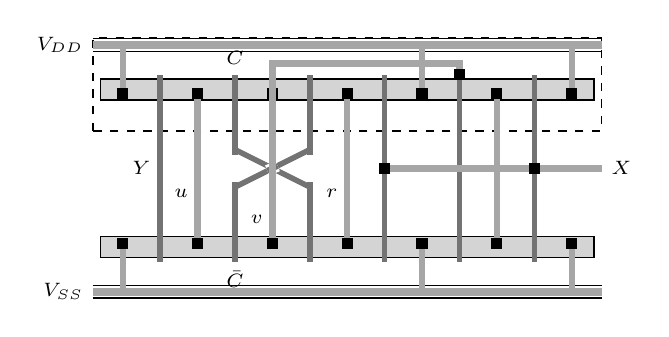
\begin{tikzpicture}[x=.95cm,y=.95cm,font=\scriptsize,line width=.5pt]
\draw[dashed] (-.4,.5) rectangle (6.4,1.75);
\begin{scope}[yshift=1cm]\VLSIDiff{-.3}{6.3}\end{scope}
\begin{scope}[yshift=-1cm]\VLSIDiff{-.3}{6.3}\end{scope}
\VLSIRail{-.4}{6.4}{1.65}\VLSIRail{-.4}{6.4}{-1.65}
\node[left] at (-.4,1.65) {$V_{DD}$};\node[left] at (-.4,-1.65) {$V_{SS}$};
% Six physical columns. Gate 1=Y; gate 2=C/Cbar; gate 3=Cbar/C;
% gate 4=X; gate 5=v; gate 6=X. Split clock gates are not shorted.
\foreach \x in {.5,3.5,4.5,5.5}{\draw[line width=2pt,black!55] (\x,-1.25)--(\x,1.25);}
\foreach \x in {1.5,2.5}{\draw[line width=2pt,black!55] (\x,.18)--(\x,1.25) (\x,-.18)--(\x,-1.25);}
\node[left] at (.5,0) {$Y$};\node[above] at (1.5,1.25) {$C$};\node[below] at (1.5,-1.25) {$\bar C$};
\draw[line width=2pt,black!55] (1.5,-.25)--(2.5,.25);\draw[line width=2pt,black!55] (1.5,.25)--(2.5,-.25);
% Opposite clock routes cross without a contact, shown with a bridge gap.
\draw[white,line width=4pt] (1.93,-.03)--(2.07,.03);\draw[line width=2pt,black!55] (1.93,-.03)--(2.07,.03);
% Supply contacts at physical channel intervals 0, 4, 6.
\foreach \x in {0,4,6}{\draw[line width=2.3pt,black!35] (\x,1)--(\x,1.65) (\x,-1)--(\x,-1.65);\VLSIContact{\x}{1}\VLSIContact{\x}{-1}}
% Inverter output u / transmission node v / feedback output r / X.
\foreach \x in {1,2,3,5}{\draw[line width=2.3pt,black!35] (\x,1)--(\x,-1);\VLSIContact{\x}{1}\VLSIContact{\x}{-1}}
\draw[line width=2.3pt,black!35] (2,.8)--(2,1.4)--(4.5,1.4)--(4.5,1.25);\VLSIContact{4.5}{1.25}
\draw[line width=2.3pt,black!35] (5,0)--(6.4,0) (3.5,0)--(5.5,0);\VLSIContact{3.5}{0}\VLSIContact{5.5}{0}
\node[right] at (6.4,0) {$X$};\node[below left] at (1,-.15) {$u$};\node[below left] at (2,-.5) {$v$};\node[below left] at (3,-.15) {$r$};
\end{tikzpicture}}
\newcommand{\OriginalLayoutB}{%
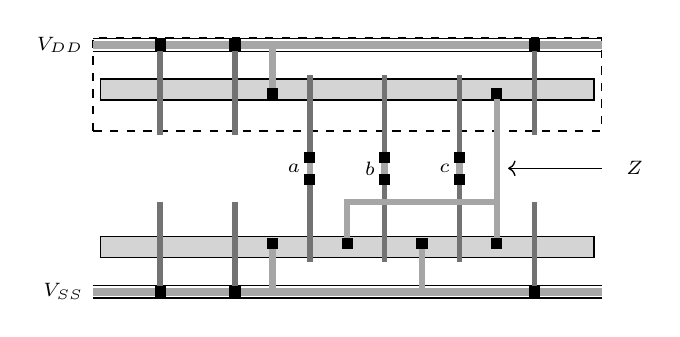
\begin{tikzpicture}[x=.95cm,y=.95cm,font=\scriptsize,line width=.5pt]
\draw[dashed] (-.4,.5) rectangle (6.4,1.75);
\begin{scope}[yshift=1cm]\VLSIDiff{-.3}{6.3}\end{scope}
\begin{scope}[yshift=-1cm]\VLSIDiff{-.3}{6.3}\end{scope}
\VLSIRail{-.4}{6.4}{1.65}\VLSIRail{-.4}{6.4}{-1.65}
\node[left] at (-.4,1.65) {$V_{DD}$};\node[left] at (-.4,-1.65) {$V_{SS}$};
\foreach \x in {.5,1.5,5.5}{\draw[line width=2pt,black!55] (\x,.45)--(\x,1.65) (\x,-.45)--(\x,-1.65);\VLSIContact{\x}{1.65}\VLSIContact{\x}{-1.65}}
\foreach \x/\g in {2.5/a,3.5/b,4.5/c}{\draw[line width=2pt,black!55] (\x,-1.25)--(\x,1.25);\draw[line width=2.3pt,black!35] (\x,-.15)--(\x,.15);\VLSIContact{\x}{-.15}\VLSIContact{\x}{.15}\node[left] at (\x,0) {$\g$};}
\draw[line width=2.3pt,black!35] (2,1)--(2,1.65) (2,-1)--(2,-1.65) (4,-1)--(4,-1.65);
\VLSIContact{2}{1}\VLSIContact{2}{-1}\VLSIContact{4}{-1}
\draw[line width=2.3pt,black!35] (5,1)--(5,-1) (3,-1)--(3,-.45)--(5,-.45);
\VLSIContact{5}{1}\VLSIContact{5}{-1}\VLSIContact{3}{-1}
\node[right] at (6.6,0) {$Z$};\draw[->] (6.4,0)--(5.15,0);
\end{tikzpicture}}

\newcommand{\SolutionLayoutA}{%
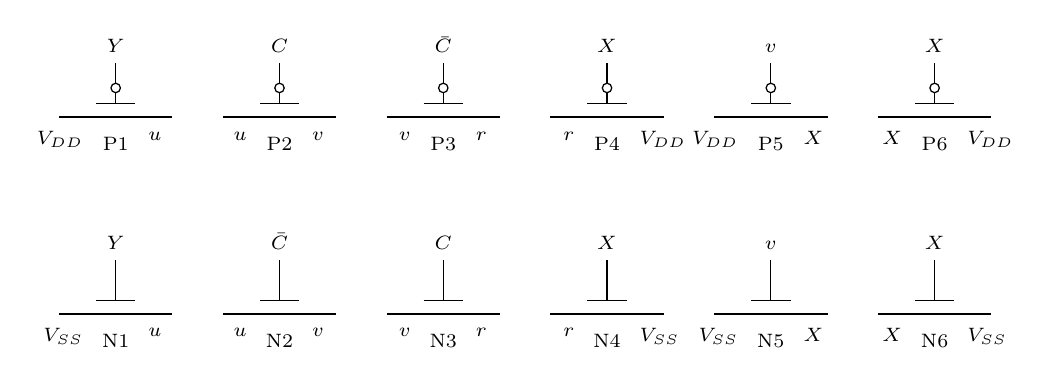
\begin{tikzpicture}[x=1cm,y=1cm,font=\scriptsize,line width=.45pt]
\draw (-0.72,2.5)--(-0.24,2.5) (0.24,2.5)--(0.72,2.5);
\draw[line width=1pt] (-0.24,2.5)--(0.24,2.5);
\draw (-0.25,2.67)--(0.25,2.67);
\draw (0.0,2.67)--(0.0,2.81);\draw (0.0,2.87) circle (.06);\draw (0.0,2.93)--(0.0,3.19);
\node[above] at (0.0,3.19) {$ Y $};
\node[below] at (0.0,2.37) {P1};
\node[anchor=north east] at (-0.29,2.44) {$ V_{DD} $};
\node[anchor=north west] at (0.29,2.44) {$ u $};
\draw (-0.72,0)--(-0.24,0) (0.24,0)--(0.72,0);
\draw[line width=1pt] (-0.24,0)--(0.24,0);
\draw (-0.25,0.17)--(0.25,0.17);
\draw (0.0,0.17)--(0.0,0.69);
\node[above] at (0.0,0.69) {$ Y $};
\node[below] at (0.0,-0.13) {N1};
\node[anchor=north east] at (-0.29,-0.06) {$ V_{SS} $};
\node[anchor=north west] at (0.29,-0.06) {$ u $};
\draw (1.36,2.5)--(1.84,2.5) (2.3200000000000003,2.5)--(2.8,2.5);
\draw[line width=1pt] (1.84,2.5)--(2.3200000000000003,2.5);
\draw (1.83,2.67)--(2.33,2.67);
\draw (2.08,2.67)--(2.08,2.81);\draw (2.08,2.87) circle (.06);\draw (2.08,2.93)--(2.08,3.19);
\node[above] at (2.08,3.19) {$ C $};
\node[below] at (2.08,2.37) {P2};
\node[anchor=north east] at (1.79,2.44) {$ u $};
\node[anchor=north west] at (2.37,2.44) {$ v $};
\draw (1.36,0)--(1.84,0) (2.3200000000000003,0)--(2.8,0);
\draw[line width=1pt] (1.84,0)--(2.3200000000000003,0);
\draw (1.83,0.17)--(2.33,0.17);
\draw (2.08,0.17)--(2.08,0.69);
\node[above] at (2.08,0.69) {$ \bar C $};
\node[below] at (2.08,-0.13) {N2};
\node[anchor=north east] at (1.79,-0.06) {$ u $};
\node[anchor=north west] at (2.37,-0.06) {$ v $};
\draw (3.4400000000000004,2.5)--(3.92,2.5) (4.4,2.5)--(4.88,2.5);
\draw[line width=1pt] (3.92,2.5)--(4.4,2.5);
\draw (3.91,2.67)--(4.41,2.67);
\draw (4.16,2.67)--(4.16,2.81);\draw (4.16,2.87) circle (.06);\draw (4.16,2.93)--(4.16,3.19);
\node[above] at (4.16,3.19) {$ \bar C $};
\node[below] at (4.16,2.37) {P3};
\node[anchor=north east] at (3.87,2.44) {$ v $};
\node[anchor=north west] at (4.45,2.44) {$ r $};
\draw (3.4400000000000004,0)--(3.92,0) (4.4,0)--(4.88,0);
\draw[line width=1pt] (3.92,0)--(4.4,0);
\draw (3.91,0.17)--(4.41,0.17);
\draw (4.16,0.17)--(4.16,0.69);
\node[above] at (4.16,0.69) {$ C $};
\node[below] at (4.16,-0.13) {N3};
\node[anchor=north east] at (3.87,-0.06) {$ v $};
\node[anchor=north west] at (4.45,-0.06) {$ r $};
\draw (5.5200000000000005,2.5)--(6.0,2.5) (6.48,2.5)--(6.96,2.5);
\draw[line width=1pt] (6.0,2.5)--(6.48,2.5);
\draw (5.99,2.67)--(6.49,2.67);
\draw (6.24,2.67)--(6.24,2.81);\draw (6.24,2.87) circle (.06);\draw (6.24,2.93)--(6.24,3.19);
\node[above] at (6.24,3.19) {$ X $};
\node[below] at (6.24,2.37) {P4};
\node[anchor=north east] at (5.95,2.44) {$ r $};
\node[anchor=north west] at (6.53,2.44) {$ V_{DD} $};
\draw (5.5200000000000005,0)--(6.0,0) (6.48,0)--(6.96,0);
\draw[line width=1pt] (6.0,0)--(6.48,0);
\draw (5.99,0.17)--(6.49,0.17);
\draw (6.24,0.17)--(6.24,0.69);
\node[above] at (6.24,0.69) {$ X $};
\node[below] at (6.24,-0.13) {N4};
\node[anchor=north east] at (5.95,-0.06) {$ r $};
\node[anchor=north west] at (6.53,-0.06) {$ V_{SS} $};
\draw (7.6000000000000005,2.5)--(8.08,2.5) (8.56,2.5)--(9.040000000000001,2.5);
\draw[line width=1pt] (8.08,2.5)--(8.56,2.5);
\draw (8.07,2.67)--(8.57,2.67);
\draw (8.32,2.67)--(8.32,2.81);\draw (8.32,2.87) circle (.06);\draw (8.32,2.93)--(8.32,3.19);
\node[above] at (8.32,3.19) {$ v $};
\node[below] at (8.32,2.37) {P5};
\node[anchor=north east] at (8.030000000000001,2.44) {$ V_{DD} $};
\node[anchor=north west] at (8.61,2.44) {$ X $};
\draw (7.6000000000000005,0)--(8.08,0) (8.56,0)--(9.040000000000001,0);
\draw[line width=1pt] (8.08,0)--(8.56,0);
\draw (8.07,0.17)--(8.57,0.17);
\draw (8.32,0.17)--(8.32,0.69);
\node[above] at (8.32,0.69) {$ v $};
\node[below] at (8.32,-0.13) {N5};
\node[anchor=north east] at (8.030000000000001,-0.06) {$ V_{SS} $};
\node[anchor=north west] at (8.61,-0.06) {$ X $};
\draw (9.68,2.5)--(10.16,2.5) (10.64,2.5)--(11.120000000000001,2.5);
\draw[line width=1pt] (10.16,2.5)--(10.64,2.5);
\draw (10.15,2.67)--(10.65,2.67);
\draw (10.4,2.67)--(10.4,2.81);\draw (10.4,2.87) circle (.06);\draw (10.4,2.93)--(10.4,3.19);
\node[above] at (10.4,3.19) {$ X $};
\node[below] at (10.4,2.37) {P6};
\node[anchor=north east] at (10.110000000000001,2.44) {$ X $};
\node[anchor=north west] at (10.69,2.44) {$ V_{DD} $};
\draw (9.68,0)--(10.16,0) (10.64,0)--(11.120000000000001,0);
\draw[line width=1pt] (10.16,0)--(10.64,0);
\draw (10.15,0.17)--(10.65,0.17);
\draw (10.4,0.17)--(10.4,0.69);
\node[above] at (10.4,0.69) {$ X $};
\node[below] at (10.4,-0.13) {N6};
\node[anchor=north east] at (10.110000000000001,-0.06) {$ X $};
\node[anchor=north west] at (10.69,-0.06) {$ V_{SS} $};
\end{tikzpicture}}
\newcommand{\SolutionLayoutB}{%
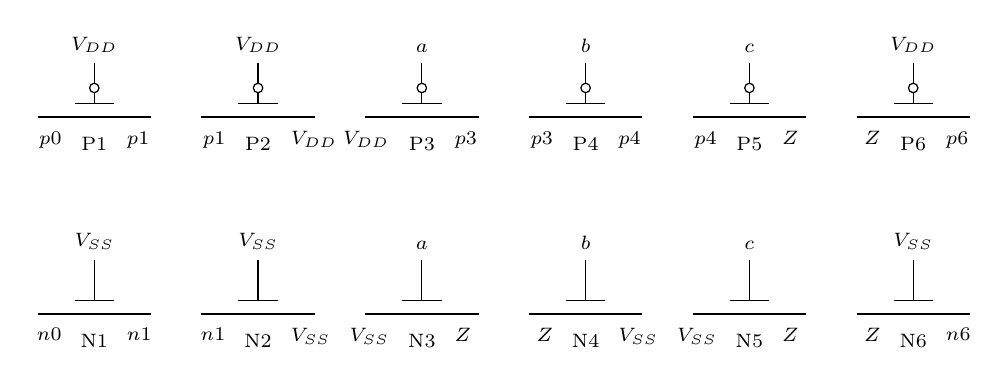
\begin{tikzpicture}[x=1cm,y=1cm,font=\scriptsize,line width=.45pt]
\draw (-0.72,2.5)--(-0.24,2.5) (0.24,2.5)--(0.72,2.5);
\draw[line width=1pt] (-0.24,2.5)--(0.24,2.5);
\draw (-0.25,2.67)--(0.25,2.67);
\draw (0.0,2.67)--(0.0,2.81);\draw (0.0,2.87) circle (.06);\draw (0.0,2.93)--(0.0,3.19);
\node[above] at (0.0,3.19) {$ V_{DD} $};
\node[below] at (0.0,2.37) {P1};
\node[anchor=north east] at (-0.29,2.44) {$ p0 $};
\node[anchor=north west] at (0.29,2.44) {$ p1 $};
\draw (-0.72,0)--(-0.24,0) (0.24,0)--(0.72,0);
\draw[line width=1pt] (-0.24,0)--(0.24,0);
\draw (-0.25,0.17)--(0.25,0.17);
\draw (0.0,0.17)--(0.0,0.69);
\node[above] at (0.0,0.69) {$ V_{SS} $};
\node[below] at (0.0,-0.13) {N1};
\node[anchor=north east] at (-0.29,-0.06) {$ n0 $};
\node[anchor=north west] at (0.29,-0.06) {$ n1 $};
\draw (1.36,2.5)--(1.84,2.5) (2.3200000000000003,2.5)--(2.8,2.5);
\draw[line width=1pt] (1.84,2.5)--(2.3200000000000003,2.5);
\draw (1.83,2.67)--(2.33,2.67);
\draw (2.08,2.67)--(2.08,2.81);\draw (2.08,2.87) circle (.06);\draw (2.08,2.93)--(2.08,3.19);
\node[above] at (2.08,3.19) {$ V_{DD} $};
\node[below] at (2.08,2.37) {P2};
\node[anchor=north east] at (1.79,2.44) {$ p1 $};
\node[anchor=north west] at (2.37,2.44) {$ V_{DD} $};
\draw (1.36,0)--(1.84,0) (2.3200000000000003,0)--(2.8,0);
\draw[line width=1pt] (1.84,0)--(2.3200000000000003,0);
\draw (1.83,0.17)--(2.33,0.17);
\draw (2.08,0.17)--(2.08,0.69);
\node[above] at (2.08,0.69) {$ V_{SS} $};
\node[below] at (2.08,-0.13) {N2};
\node[anchor=north east] at (1.79,-0.06) {$ n1 $};
\node[anchor=north west] at (2.37,-0.06) {$ V_{SS} $};
\draw (3.4400000000000004,2.5)--(3.92,2.5) (4.4,2.5)--(4.88,2.5);
\draw[line width=1pt] (3.92,2.5)--(4.4,2.5);
\draw (3.91,2.67)--(4.41,2.67);
\draw (4.16,2.67)--(4.16,2.81);\draw (4.16,2.87) circle (.06);\draw (4.16,2.93)--(4.16,3.19);
\node[above] at (4.16,3.19) {$ a $};
\node[below] at (4.16,2.37) {P3};
\node[anchor=north east] at (3.87,2.44) {$ V_{DD} $};
\node[anchor=north west] at (4.45,2.44) {$ p3 $};
\draw (3.4400000000000004,0)--(3.92,0) (4.4,0)--(4.88,0);
\draw[line width=1pt] (3.92,0)--(4.4,0);
\draw (3.91,0.17)--(4.41,0.17);
\draw (4.16,0.17)--(4.16,0.69);
\node[above] at (4.16,0.69) {$ a $};
\node[below] at (4.16,-0.13) {N3};
\node[anchor=north east] at (3.87,-0.06) {$ V_{SS} $};
\node[anchor=north west] at (4.45,-0.06) {$ Z $};
\draw (5.5200000000000005,2.5)--(6.0,2.5) (6.48,2.5)--(6.96,2.5);
\draw[line width=1pt] (6.0,2.5)--(6.48,2.5);
\draw (5.99,2.67)--(6.49,2.67);
\draw (6.24,2.67)--(6.24,2.81);\draw (6.24,2.87) circle (.06);\draw (6.24,2.93)--(6.24,3.19);
\node[above] at (6.24,3.19) {$ b $};
\node[below] at (6.24,2.37) {P4};
\node[anchor=north east] at (5.95,2.44) {$ p3 $};
\node[anchor=north west] at (6.53,2.44) {$ p4 $};
\draw (5.5200000000000005,0)--(6.0,0) (6.48,0)--(6.96,0);
\draw[line width=1pt] (6.0,0)--(6.48,0);
\draw (5.99,0.17)--(6.49,0.17);
\draw (6.24,0.17)--(6.24,0.69);
\node[above] at (6.24,0.69) {$ b $};
\node[below] at (6.24,-0.13) {N4};
\node[anchor=north east] at (5.95,-0.06) {$ Z $};
\node[anchor=north west] at (6.53,-0.06) {$ V_{SS} $};
\draw (7.6000000000000005,2.5)--(8.08,2.5) (8.56,2.5)--(9.040000000000001,2.5);
\draw[line width=1pt] (8.08,2.5)--(8.56,2.5);
\draw (8.07,2.67)--(8.57,2.67);
\draw (8.32,2.67)--(8.32,2.81);\draw (8.32,2.87) circle (.06);\draw (8.32,2.93)--(8.32,3.19);
\node[above] at (8.32,3.19) {$ c $};
\node[below] at (8.32,2.37) {P5};
\node[anchor=north east] at (8.030000000000001,2.44) {$ p4 $};
\node[anchor=north west] at (8.61,2.44) {$ Z $};
\draw (7.6000000000000005,0)--(8.08,0) (8.56,0)--(9.040000000000001,0);
\draw[line width=1pt] (8.08,0)--(8.56,0);
\draw (8.07,0.17)--(8.57,0.17);
\draw (8.32,0.17)--(8.32,0.69);
\node[above] at (8.32,0.69) {$ c $};
\node[below] at (8.32,-0.13) {N5};
\node[anchor=north east] at (8.030000000000001,-0.06) {$ V_{SS} $};
\node[anchor=north west] at (8.61,-0.06) {$ Z $};
\draw (9.68,2.5)--(10.16,2.5) (10.64,2.5)--(11.120000000000001,2.5);
\draw[line width=1pt] (10.16,2.5)--(10.64,2.5);
\draw (10.15,2.67)--(10.65,2.67);
\draw (10.4,2.67)--(10.4,2.81);\draw (10.4,2.87) circle (.06);\draw (10.4,2.93)--(10.4,3.19);
\node[above] at (10.4,3.19) {$ V_{DD} $};
\node[below] at (10.4,2.37) {P6};
\node[anchor=north east] at (10.110000000000001,2.44) {$ Z $};
\node[anchor=north west] at (10.69,2.44) {$ p6 $};
\draw (9.68,0)--(10.16,0) (10.64,0)--(11.120000000000001,0);
\draw[line width=1pt] (10.16,0)--(10.64,0);
\draw (10.15,0.17)--(10.65,0.17);
\draw (10.4,0.17)--(10.4,0.69);
\node[above] at (10.4,0.69) {$ V_{SS} $};
\node[below] at (10.4,-0.13) {N6};
\node[anchor=north east] at (10.110000000000001,-0.06) {$ Z $};
\node[anchor=north west] at (10.69,-0.06) {$ n6 $};
\end{tikzpicture}}

\begin{document}
\begin{center}{\large\bfseries EE3032 Introduction to VLSI Design -- Final}\\Fall 2013\end{center}
\textbf{Note: Total number of points is 150, but the number of points you can get is smaller than 100.} The printed note and all point labels are preserved without rescaling.

\textbf{1. (40 points)} Answer the following questions.
\begin{enumerate}[label=(\alph*),leftmargin=7mm,itemsep=2pt]
\item List two approaches which can be used to alleviate the occurrence probability of latchup. (4 points)
\item Explain the following definitions: (1) physical design, (2) instantiate a cell, and (3) instance. (6 points)
\item List two requirements which must be met when you draw the layout of a cell in the cell library. (4 points)
\item What is soft error? (2 points)
\item Why is the soft error rate of a circuit increased with increasing operation frequency and scaling down the technology process? Explain the cause in terms of logical masking effect, electrical masking effect, and latch window effect. (6 points)
\item List two methods which can be used to reduce the power bounce and ground bounce occurring in the IO pads. (4 points)
\item List two major problems of dynamic logic. (4 points)
\item List two limitations of CMOS domino logic. (4 points)
\item What are core-limited design and pad-limited design? (4 points)
\item A pseudo-NMOS logic is called a ratioed logic. Why? (2 points)
\end{enumerate}
\textbf{2. (10 points)} Sketch the Boolean function $f=\overline{AB(C+D)}$ using each of the following logic design techniques: (1) Dynamic logic (5 points) and (2) Fully differential logic (5 points).

\textbf{3. (15 points)} Figure 1 shows a domino logic gate. Assume that 0.18 $\mu$m technology is used to design the gate and $\mu_n=3\mu_p$. Also, a $2\,\mu\mathrm m/0.18\,\mu\mathrm m$ PMOS/NMOS has input capacitance $C$ (i.e., $C_g=C$). Complete the following questions.
\begin{enumerate}[label=(\alph*),leftmargin=7mm]
\item Assume that the size of P1 is $4\,\mu\mathrm m/0.18\,\mu\mathrm m$ and all channel lengths are $0.18\,\mu\mathrm m$. Determine the sizes of N1--N6 such that the rise time and fall time of node $X$ are equal, i.e., $t_r=t_f$. (5 points)
\item Your boss asks you to design the dynamic gate such that the switching power of CLK is $2fCV_{DD}^{2}$, where $f$ and $V_{DD}$ denote the operation frequency and supply voltage. Determine the sizes of N1--N6 and P1 such that the rise time and fall time of node $X$ are equal. (10 points)
\end{enumerate}
\begin{center}\begin{tikzpicture}[scale=.83,font=\scriptsize]
\mos{2}{5}{CLK}{1}\rail{2.25}{5.5}{V_{DD}}\node[right]at(2.6,5){P1};\draw(.25,4.5)--(4.25,4.5);\node[above]at(3,4.5){$X$};
\mos{0}{3}{}{0}\node[right]at(.45,3){N1};\draw(.25,3.5)--(.25,4.5);\draw(.25,2.5)--(.25,1.5);
\mos{2}{4}{}{0}\mos{2}{2}{}{0}\node[right]at(2.55,4){N2};\node[right]at(2.55,2){N3};\draw(2.25,3.5)--(2.25,2.5);
\mos{4}{4}{}{0}\mos{4}{3}{}{0}\node[right]at(4.6,4){N4};\node[right]at(4.6,3){N5};\draw(2.25,2.5)--(4.25,2.5);\fill(2.25,2.5)circle(1pt);
\draw(.25,1.5)--(2.25,1.5);\mos{2}{1}{CLK}{0}\node[right]at(2.6,1){N6};\ground{2.25}{.5}
\mos{7}{4.1}{}{1}\mos{7}{3.1}{}{0}\rail{7.25}{4.6}{V_{DD}}\ground{7.25}{2.6}\node[right]at(7.6,4.1){P2};\node[right]at(7.6,3.1){N7};\draw(4.25,4.5)--(5.8,4.5)--(5.8,3.1)--(6.25,3.1);\draw(5.8,4.1)--(6.25,4.1);\draw(7.25,3.6)--(8.4,3.6)node[right]{output};\end{tikzpicture}\\Figure 1: A dynamic logic circuit. Data gates are unlabeled as in the source.\end{center}
\newpage
\textbf{4. (15 points)} Figure 2 shows a combinational circuit designed with NP-domino logic. All NMOS have the same $\beta_n$, all PMOS have the same $\beta_p$, and $\beta_n=\beta_p$. Also $\mu_n=2\mu_p$, the PMOS/NMOS gate capacitances are $2C/C$, respectively, and each turn-on equivalent resistance is $R$.
\begin{enumerate}[label=(\alph*),leftmargin=7mm]
\item The rise/fall time is the product of the output capacitance and equivalent resistance of the output charging/discharging path, respectively. The gate delay is $t_d=(t_r+t_f)/2$, and transistor drain capacitances can be neglected. Calculate the contamination delay $t_{cd}$ and propagation delay $t_{pd}$ in terms of $R$ and $C$. (10 points)
\item Assume $V_{DD}=1.8$ V and $|V_{tp}|=0.5$ V. The capacitances of $x,y,z$ are $0.4,0.8,1.0$ pF, respectively. Can the circuit operate correctly? Explain. (5 points)
\end{enumerate}
\begin{center}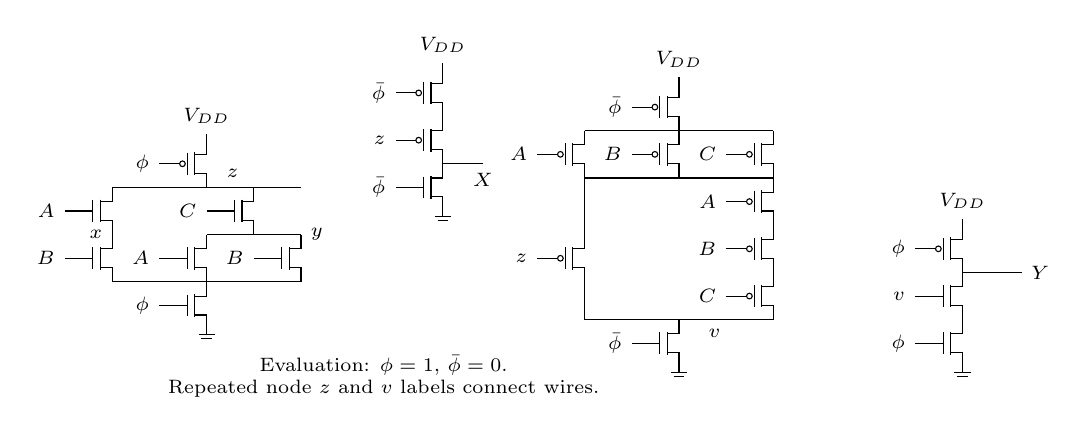
\begin{tikzpicture}[scale=.60,font=\scriptsize]
\mos{2}{5.8}{\phi}{1}\rail{2.25}{6.3}{V_{DD}}\draw(.25,5.3)--(4.25,5.3);\node[above]at(2.8,5.3){$z$};
\mos{0}{4.8}{A}{0}\mos{0}{3.8}{B}{0}\node[left]at(.25,4.3){$x$};\mos{3}{4.8}{C}{0}\draw(3.25,4.3)--(4.25,4.3);\mos{2}{3.8}{A}{0}\mos{4}{3.8}{B}{0}\draw(2.25,4.3)--(3.25,4.3);\node[right]at(4.25,4.3){$y$};\draw(.25,3.3)--(4.25,3.3);\mos{2}{2.8}{\phi}{0}\ground{2.25}{2.3}
\mos{7}{7.3}{\bar\phi}{1}\rail{7.25}{7.8}{V_{DD}}\mos{7}{6.3}{z}{1}\mos{7}{5.3}{\bar\phi}{0}\ground{7.25}{4.8}\draw(7.25,5.8)--(8.1,5.8)node[below]{$X$};
\mos{12}{7}{\bar\phi}{1}\rail{12.25}{7.5}{V_{DD}}\draw(10.25,6.5)--(14.25,6.5);\mos{10}{6}{A}{1}\mos{12}{6}{B}{1}\mos{14}{6}{C}{1}\draw(10.25,5.5)--(14.25,5.5);
\mos{10}{3.8}{z}{1}\draw(10.25,4.3)--(10.25,5.5);\draw(10.25,3.3)--(10.25,2.5)--(14.25,2.5);
\mos{14}{5}{A}{1}\mos{14}{4}{B}{1}\mos{14}{3}{C}{1}\mos{12}{2}{\bar\phi}{0}\ground{12.25}{1.5}\node[below]at(13,2.5){$v$};
\mos{18}{4}{\phi}{1}\rail{18.25}{4.5}{V_{DD}}\mos{18}{3}{v}{0}\mos{18}{2}{\phi}{0}\ground{18.25}{1.5}\draw(18.25,3.5)--(19.5,3.5)node[right]{$Y$};
\node[align=center]at(6,1.3){Evaluation: $\phi=1$, $\bar\phi=0$.\\Repeated node $z$ and $v$ labels connect wires.};\end{tikzpicture}\\Figure 2: A circuit designed with NP-domino logic.\end{center}
\textbf{5. (25 points)} Figure 3 shows a sequential circuit. The register clock-to-Q propagation delay, clock-to-Q contamination delay, setup time and hold time are $0.3,0.1,0.2,0.4$ ns, respectively. The NOR, XOR, XNOR and inverter delays are $0.2,0.5,0.4,0.2$ ns, respectively.
\begin{enumerate}[label=(\alph*),leftmargin=7mm]
\item If clock skew is 0 ns, can the circuit operate correctly? If not, modify the circuit so that it can operate correctly without sacrificing operation frequency. (5 points)
\item If clock skew is 0 ns, determine the maximum operation frequency. (5 points)
\item If clock skew is 0.5 ns, determine the maximum operation frequency. (5 points)
\item If you can insert three additional registers to boost the operation frequency, where should they be inserted so that maximum improvement is achieved? Draw the modified circuit and calculate its maximum delay. (10 points)
\end{enumerate}
\begin{center}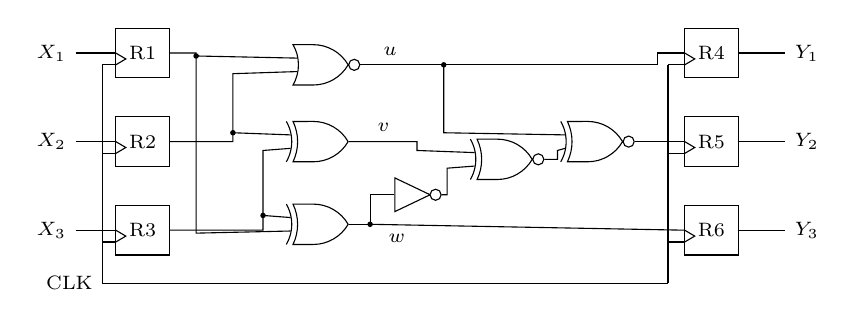
\begin{tikzpicture}[x=.85cm,y=.75cm,font=\scriptsize]
\foreach\i/\y in {1/4,2/2.5,3/1}{\draw(0,\y-.42)rectangle(.8,\y+.42);\node at(.4,\y){R\i};\draw(0,\y-.2)--(.15,\y-.1)--(0,\y);\draw(-.6,\y)--(0,\y)node[pos=0,left]{$X_\i$};}
\foreach\i/\y/\j in {4/4/1,5/2.5/2,6/1/3}{\draw(8.5,\y-.42)rectangle(9.3,\y+.42);\node at(8.9,\y){R\i};\draw(8.5,\y-.2)--(8.65,\y-.1)--(8.5,\y);\draw(9.3,\y)--(10,\y)node[right]{$Y_\j$};}
\node[nor gate US,draw,logic gate inputs=nn,minimum width=.7cm](u)at(3,3.8){};\node[xor gate US,draw,logic gate inputs=nn,minimum width=.7cm](v)at(3,2.5){};\node[xor gate US,draw,logic gate inputs=nn,minimum width=.7cm](w)at(3,1.1){};\node[not gate US,draw,minimum width=.5cm](n)at(4.35,1.6){};\node[xnor gate US,draw,logic gate inputs=nn,minimum width=.7cm](s)at(5.75,2.2){};\node[xnor gate US,draw,logic gate inputs=nn,minimum width=.7cm](o)at(7.1,2.5){};
\draw(.8,4)--(1.2,4)--(1.2,3.95)--(u.input 1);\draw(1.2,3.95)--(1.2,.95)--(w.input 2);\fill(1.2,3.95)circle(1pt);
\draw(.8,2.5)--(1.75,2.5)--(1.75,2.65)--(v.input 1);\draw(1.75,2.65)--(1.75,3.65)--(u.input 2);\fill(1.75,2.65)circle(1pt);
\draw(.8,1)--(2.2,1)--(2.2,1.25)--(w.input 1);\draw(2.2,1.25)--(2.2,2.35)--(v.input 2);\fill(2.2,1.25)circle(1pt);
\draw(u.output)--(8.1,3.8)--(8.1,4)--(8.5,4);\draw(4.9,3.8)--(4.9,2.65)--(o.input 1);\fill(4.9,3.8)circle(1pt);\node[above]at(4.1,3.8){$u$};
\draw(v.output)--(4.5,2.5)--(4.5,2.35)--(s.input 1);\node[above]at(4,2.5){$v$};\draw(w.output)--(3.8,1.1)--(3.8,1.6)--(n.input);\draw(3.8,1.1)--(8.5,1);\fill(3.8,1.1)circle(1pt);\node[below]at(4.2,1.1){$w$};\draw(n.output)--(4.95,1.6)--(4.95,2.05)--(s.input 2);\draw(s.output)--(6.6,2.2)--(6.6,2.35)--(o.input 2);\draw(o.output)--(8.5,2.5);
\draw(-.2,.1)node[left]{CLK}--(8.25,.1);\draw(-.2,.1)--(-.2,3.8);\draw(8.25,.1)--(8.25,3.8);\foreach\y in {3.8,2.3,.8}{\draw(-.2,\y)--(0,\y);\draw(8.25,\y)--(8.5,\y);}\end{tikzpicture}\\Figure 3: A sequential circuit.\end{center}
\newpage
\textbf{6. (20 points)} Figure 4 shows two symbolic layouts of two circuits. Draw the transistor-level schematic diagrams of the two circuits.
\begin{center}\OriginalLayoutA\quad\OriginalLayoutB\\Figure 4: Symbolic layouts of two circuits: (a) left, (b) right.\end{center}
\textbf{7. (10 points)} Figure 5 shows a Schmitt circuit, where $V_{tn}=|V_{tp}|=0.6$ V. If an input signal as shown in the left figure is applied, the circuit outputs the signal shown in the right figure. Derive the ratios $\beta_{N1}/\beta_{N3}$ and $\beta_{P1}/\beta_{P3}$.
\begin{center}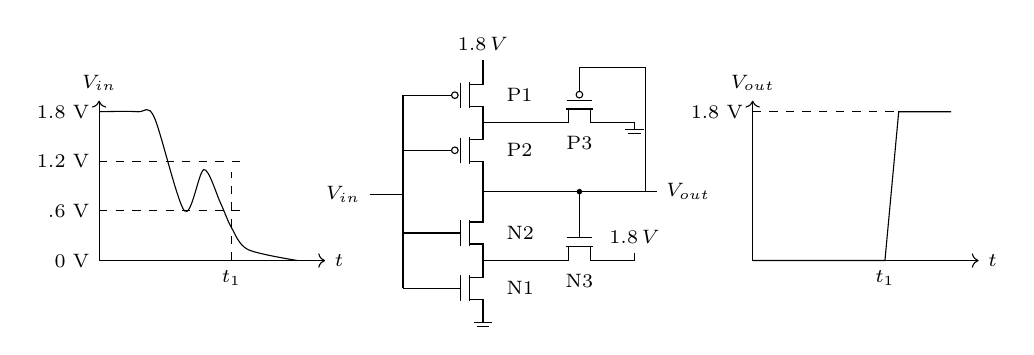
\begin{tikzpicture}[x=.7cm,y=.7cm,font=\scriptsize]
\draw[->](0,0)--(4.1,0)node[right]{$t$};\draw[->](0,0)--(0,2.9)node[above]{$V_{in}$};\foreach\y/\v in {0/0,.9/.6,1.8/1.2,2.7/1.8}{\node[left]at(0,\y){$\v$ V};}\draw[dashed](0,.9)--(2.6,.9);\draw[dashed](0,1.8)--(2.6,1.8);\draw plot[smooth]coordinates{(0,2.7)(.7,2.7)(1,2.6)(1.55,.9)(1.9,1.65)(2.2,1.05)(2.4,.6)(2.7,.2)(3.6,0)};\draw[dashed](2.4,0)--(2.4,1.6);\node[below]at(2.4,0){$t_1$};
\begin{scope}[xshift=4cm]\mos{1}{3}{}{1}\mos{1}{2}{}{1}\mos{1}{.5}{}{0}\mos{1}{-.5}{}{0}\rail{1.25}{3.5}{1.8\,V}\ground{1.25}{-1}\draw(1.25,1)--(1.25,1.5);\draw(1.25,1.25)--(4.4,1.25)node[right]{$V_{out}$};\draw(-.2,-.5)--(-.2,3)--(.25,3);\foreach\y in {2,.5,-.5}{\draw(-.2,\y)--(.25,\y);}\draw(-.8,1.2)node[left]{$V_{in}$}--(-.2,1.2);\node[right]at(1.5,3){P1};\node[right]at(1.5,2){P2};\node[right]at(1.5,.5){N2};\node[right]at(1.5,-.5){N1};
\hmos{3}{2.75}{P3}{1}\draw(1.25,2.5)--(2.5,2.5);\draw(3.5,2.5)--(4,2.5);\ground{4}{2.5}\draw(3,3.5)--(4.2,3.5)--(4.2,1.25);\hmos{3}{.25}{N3}{0}\draw(1.25,0)--(2.5,0);\draw(3.5,0)--(4,0);\rail{4}{0}{1.8\,V}\draw(3,1)--(3,1.25);\fill(3,1.25)circle(1pt);\end{scope}
\begin{scope}[xshift=8.3cm]\draw[->](0,0)--(4.1,0)node[right]{$t$};\draw[->](0,0)--(0,2.9)node[above]{$V_{out}$};\node[left]at(0,2.7){1.8 V};\draw[dashed](0,2.7)--(3.3,2.7);\draw(0,0)--(2.4,0)--(2.65,2.7)--(3.6,2.7);\node[below]at(2.4,0){$t_1$};\end{scope}\end{tikzpicture}\\Figure 5: A CMOS Schmitt circuit.\end{center}
\textbf{8. (15 points)} Figure 6 shows a register realized by two low-cost latches. Complete the following questions.
\begin{enumerate}[label=(\alph*),leftmargin=7mm]
\item What type of register is it? Explain. (5 points)
\item Assume that the switching threshold of inverter Inv1 is $V_{DD}/2$, and the turn-on equivalent resistances of the transmission gate, N1, N2, P1 and P2 are $R_{TG},R_{N1},R_{N2},R_{P1},R_{P2}$, respectively. List two inequalities for determining the sizes of P2 and N2 such that the register can operate correctly. (10 points)
\end{enumerate}
\begin{center}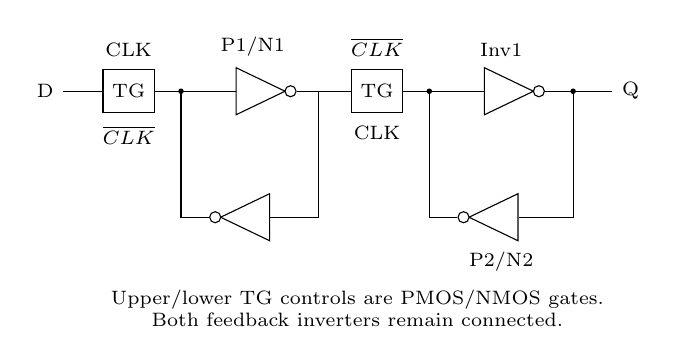
\begin{tikzpicture}[x=.83cm,y=.8cm,font=\scriptsize]
\node[draw,minimum width=.6cm,minimum height=.55cm](t1)at(.7,2.5){TG};\draw(-.3,2.5)node[left]{D}--(t1.west);\node[above]at(.7,2.9){CLK};\node[below]at(.7,2.1){$\overline{CLK}$};
\node[not gate US,draw,minimum width=.7cm](i1)at(2.6,2.5){};\draw(t1.east)--(i1.input);\node[above]at(2.6,2.9){P1/N1};\node[not gate US,draw,rotate=180,minimum width=.7cm](f1)at(2.6,.5){};\draw(i1.output)--(3.6,2.5)--(3.6,.5)--(f1.input);\draw(f1.output)--(1.5,.5)--(1.5,2.5);\fill(1.5,2.5)circle(1pt);
\node[draw,minimum width=.6cm,minimum height=.55cm](t2)at(4.5,2.5){TG};\draw(3.6,2.5)--(t2.west);\node[above]at(4.5,2.9){$\overline{CLK}$};\node[below]at(4.5,2.1){CLK};
\node[not gate US,draw,minimum width=.7cm](i2)at(6.4,2.5){};\draw(t2.east)--(i2.input);\node[above]at(6.4,2.9){Inv1};\draw(i2.output)--(8.1,2.5)node[right]{Q};\node[not gate US,draw,rotate=180,minimum width=.7cm](f2)at(6.4,.5){};\node[below]at(6.4,.1){P2/N2};\draw(7.5,2.5)--(7.5,.5)--(f2.input);\draw(f2.output)--(5.3,.5)--(5.3,2.5);\fill(5.3,2.5)circle(1pt);\fill(7.5,2.5)circle(1pt);\node[align=center]at(4.2,-.95){Upper/lower TG controls are PMOS/NMOS gates.\\Both feedback inverters remain connected.};\end{tikzpicture}\\Figure 6: A register consisting of two low-cost latches.\end{center}
\small Reconstruction notes: This reconstruction covers the dated three-page paper. All reconstructed figures are editable vectors. Identical 2012 figures were consulted only for low-resolution circuit/contact details; 2013 wording, numbers and points govern.\end{document}
